\chapter{Case Study 2 (Liar's Dice)}

In this case study, we introduce Liar's Dice, a dice game utilising hidden information. We introduce partially observable MDPs (known as POMDPs) to represent this hidden information, model a small version of the game using a POMDP, and analyse the susceptibility of Liar's Dice to the snowball effect.

\section{Liar's Dice description}
Liar's Dice is a dice game for multiple players, where each player must be able to bluff and detect opponent's bluffs in order to win. Liar's Dice takes place over a series of rounds, where each player rolls their dice, keeping the values on the dice hidden from other players. A player then makes a \emph{bid}, which is comprised of a face value ono a dice, and the number of dice that show that value. Players then rotate in turn, choosing to either make a higher bid (with either a higher face value, a higher quantity, or both), or challenge the previous bid. If a challenge is made, all dice are revealed. If the bid was correct, the challenging player loses a die. If the bid was incorrect, the bidding player loses a die. The player who lost starts the next round, and play continues until only one player has any remaining dice.

In Liar's Dice, every player starts with the same amount of information, since every player starts with the same number of dice. However, as the game progresses, some players will have more dice than others, changing bidding behaviour, as demonstrated by the following example:

\begin{example}
\label{cs2:hidden_info_example}

Consider the situation presented in Figure \ref{cs2:uneven_information}, where the first player has rolled two 2s while the second player has rolled a 5. The first player can confidently make a bid that there are two 2s, but the second player cannot see enough dice to determine the correctness of this bid. Hence, the second player has three options:

\begin{itemize}

\item If the second player challenges the bid, they will lose a dice, and therefore lose the game.
\item If the second player increases the face value of the bid, then the first player can immediately challenge the bid and win the game, since they know that at most one dice cannot have value 2.
\item If the second player increases the quantity of the bid, to bidding that there are three 2s, the first player can challenge and win with probability $\frac{5}{6}$.

\end{itemize}

As a result, the first player is able to use their increased access to information in order to increase their chances of success.

\end{example}

\begin{figure}[h]
    \centering
    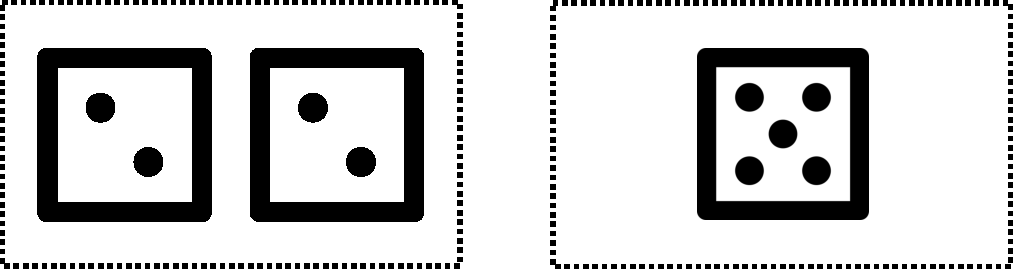
\includegraphics[width=0.7\textwidth]{images/LiarsDice/different_information.pdf}
    \caption{A game of Liar's Dice, where the first player has rolled two 2s while the second player has rolled a 5.}
    \label{cs2:uneven_information}
\end{figure}

This example represents a potential issue with the design of Liar's Dice. Initially we expect that the probability of either player losing a round is even, depending primarily on the strategies the players employ. However, as the game progresses, players with fewer dice are more likely to lose subsequent rounds, making it harder and harder for players to win from behind, a phenomenon known as the \emph{snowball effect} in game design. 

In particular, the snowball effect means that the overall results of games may be decided fairly early on, even if the games are long. This is frustrating for players - the players are still required to play several rounds of a game where the result is already a foregone conclusion. Moreover, with multiple players, this presents an opportunity for one player to be eliminated very early, since the game continues without their involvement.

Our aim when analysing Shut the Box will be to examine to what extent Liar's Dice exhibits the snowball effect, and whether this effect can be mitigated in some way. Firstly, we introduce a variant of MDPs which allows for partial observability, in order to model the hidden information present in Liar's Dice.

\section{Background (1 page)}

A key aspect of Liar's Dice is partial observability, which we now introduce in order to augment our existing MDPs, as described in \cite{norman_verification_2017}.

\begin{definition}
    \label{cs2:def-pomdps}

    A partially observable Markov decision process (or POMDP) is a tuple $\mathcal{P} = (S, \bar{s}, A, \delta, L, \mathcal{O}, obs)$ such that:

    \begin{itemize}
        \item $(S, \bar{s}, A, \delta, L)$ is an MDP, as in Definition \ref{cs1:def_mdps}.
        \item $\mathcal{O}$ is a finite set of \emph{observations}
        \item $obs : S \rightarrow 2^{\mathcal{O}}$ labels each state with a subset of observations.
        \item For any two states $s, s' \in S$, if $obs(s) = obs(s')$ then the available actions at $s$ and $s'$ must be identical. When this occurs, we say that states $s$ and $s'$ are \emph{observationally equivalent}
    \end{itemize}
\end{definition}

The last point in this definition indicates how POMDPs can represent hidden information. Rather than being able to directly access every state, decisions can only be made based on observations. For instance, in many card games, some cards may be visible for a particular player, while others are hidden. In order for two states to be observationally equivalent in a model of this game, we only require that the visible cards are the same in both states, while the hidden cards can range across any permutation of valid cards.

Since POMDPs are an extension of an MDP, adversaries for POMDPs are defined in terms of adversaries for the corresponding MDP. However, in order to reflect the added constraints that observations provide, we require that adversaries on observationally equivalent paths are equivalent:

\begin{definition}
\label{cs1:pomdp_strats}

For a POMDP $P$, an adversary of $P$ is a function $\sigma$ mapping all finite paths through the POMDP to a discrete probability distribution over the set of actions. In particular, $\sigma$ is also an adversary of the corresponding MDP. Moreover, for paths $\pi = s_0 \xrightarrow{a_0} s_1 \xrightarrow{a_1} \dots s_n$ and $\pi = s'_0 \xrightarrow{a'_0} s'_1 \xrightarrow{a'_1} \dots s'_n$, if $obs(s_i) = obs(s'_i)$ and $a_i = a'_i$ for all $i \in \mathbb{N}$, then $\sigma(\pi) = \sigma(\pi')$. In other words, $\sigma$ makes the same decisions in observationally equivalent paths.

\end{definition}

This definition references a key difference in optimal adversary generation between MDPs and POMDPs. In MDPs, optimal adversaries are deterministic and memoryless, so in particular adversaries map states to actions. This allows for aforementioned methods such as value iteration to be applied, allowing for efficient computation of optimal values and adversaries attaining these optimal values.





Describe POMDPs here - what makes them important and useful compared to MDPs? Explain why we add this additional complexity, but also mention trade offs in terms of the sorts of analysis we can perform.


\section{Analysis (3 pages)}

Collect data, show results. Make sure to mention how game trees are constructed to infer results about games based on individual rounds.


\section{Evaluation (2 pages)}

Again, use model checking results to answer questions about Liar's Dice. Discuss potential limitations of analysis that arise from using POMDPs.

